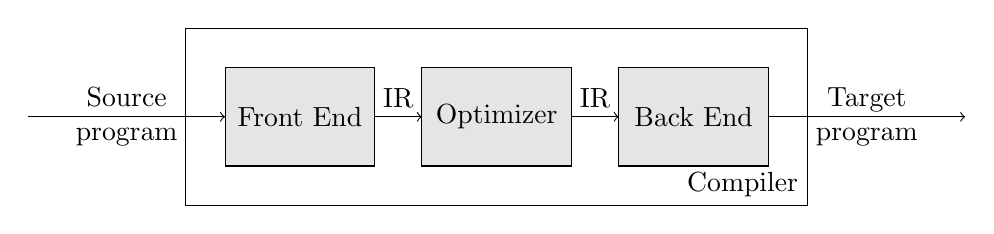
\begin{tikzpicture}
    \draw (-0.5, -0.5) rectangle ++(7.9, 2.25) node[anchor=north east, yshift=-1.7cm]{Compiler};
    \filldraw[fill=gray!20] (0,0) rectangle ++(1.9, 1.25) node[pos=.5]{Front End};
    \filldraw[fill=gray!20] (2.5,0) rectangle ++(1.9, 1.25) node[pos=.5]{Optimizer};
    \filldraw[fill=gray!20] (5,0) rectangle ++(1.9, 1.25) node[pos=.5]{Back End};
    \draw[->] (1.9, 0.625) -- ++(0.6, 0) node[midway, above]{IR};
    \draw[->] (4.4, 0.625) -- ++(0.6, 0) node[midway, above]{IR};
    \draw[->] (-2.5, 0.625) -- ++(2.5, 0) node[midway, align=center]{Source \\ program};
    \draw[->] (6.9, 0.625) -- ++(2.5, 0) node[midway, align=center]{Target \\ program};
\end{tikzpicture}